\documentclass{article}

\usepackage[margin=1in]{geometry}

\usepackage{amsmath}
\usepackage{amssymb}
\usepackage{calc}
\usepackage{caption}
\usepackage{graphicx}
\usepackage{indentfirst}
\usepackage{lmodern}
\usepackage{newfloat}
\usepackage[dvipsnames]{xcolor}
\usepackage{tikz, tikz-qtree}
\usepackage[utf8]{inputenc}
\usepackage[T1]{fontenc}
\usepackage[normalem]{ulem}
\usepackage[hidelinks]{hyperref}


\setlength{\parskip}{5pt}%

\DeclareFloatingEnvironment[fileext=lod]{diagram}
\captionsetup[diagram]{labelformat=empty}
\captionsetup[figure]{labelformat=empty}

\usetikzlibrary{trees}
\usetikzlibrary{positioning}
\tikzset{level distance=45pt}
\tikzset{
  edge from parent/.style= { draw, edge from parent path= {
      (\tikzparentnode.south)
      -- +(0,-15pt)
      -| (\tikzchildnode)
    }
  }
}


\begin{document}

\begin{titlepage}
  \centering
  
  \vfill{
    \bfseries\Huge
    Universidade Federal de Minas Gerais\\[5pt]
    \bfseries\Large
    Bacharel em Sistemas de Informação \\
    Algoritmos e Estruturas de Dados 3\\
  }
  
  \vfill
  
  \includegraphics[width=13cm]{images/ufmg_logo.jpg}
  
  \vfill{
    \bfseries\Large
    Trabalho Prático 1\\
    Agosto 2017\\
  }
  \vfill{
    \bfseries\large
    Gabriel Silva Bastos\\[5pt]
    Matrícula: 2016058204
  }
\end{titlepage}


\section{Introdução}
O objetivo do trabalho é prover uma comparação que evidencie os ganhos de eficiência ao se estruturar dados de forma inteligente. Para tal, foi proposto um problema e duas formas de se resolver o mesmo. O problema consiste em obter informações sobre máximos, mínimos e somas em intervalos de um vetor mutável. A primeira solução consiste em estruturar os dados de forma trivial, Já a segunda solução implementa uma estruturação mais elaborada. Desta forma, será feita a comparação da eficiência de ambas soluções.


\section{Visão Geral das Soluções}
Tendo como entrada um vetor de $n$ números, ambas soluções são formas de se pré-computar triplas contendo o mínimo, máximo e a soma dos elementos em dado intervalo $[i, j]$ contido no vetor.
\[ T_{i,j} = {(\text{Min}, \text{Max}, \text{Soma})}_{i,j} \]

\subsection{Matriz}
Uma matriz foi escolhida como forma trivial de se estruturar os dados. Cada entrada na posição $i, j$ na matriz contém a tupla correspondente ao intervalo $[i,j]$.
\[
  \begin{bmatrix}
      T_{1,1} & \hdots  & T_{1,n} \\
      \vdots & \ddots  & \vdots \\
      T_{n,1} & \hdots & T_{n,n}
  \end{bmatrix}
\]
Para se obter a tripla de um certo intervalo, uma simples consulta na matriz é suficiente. \\
Para cada alteração no vetor, a matriz deve ser reconstruida.

\subsection{Árvore de Segmentos}
Uma árvore de segmentos foi escolhida como forma elaborada de se estruturar os dados. Cada nó na arvóre representa um intervalo. As folhas representam todos intervalos de largura $1$, já os nós internos representam o intervalo resultante da união dos intervalos de seus descendentes. A raiz representa o intervalo correspondente a todo o vetor.
\begin{diagram}[h]
  \centering
  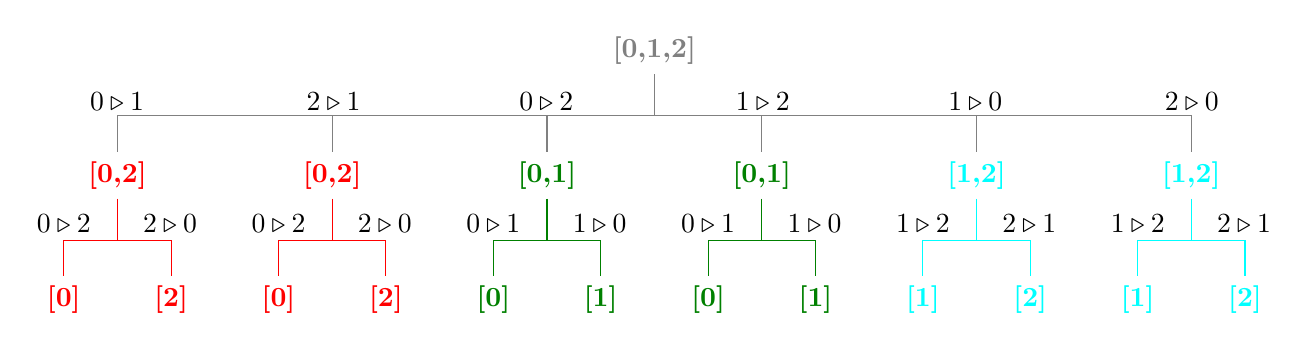
\begin{tikzpicture}[sibling distance=20pt]
    \tikzset{every tree node/.style={font=\bf}}
    \Tree [
      .\node[text=gray] (root) {[0,1,2]};
          \edge[draw=gray]; [.\node[text=Red] (s1) {[0,2]}; \edge[draw=Red]; {\color{Red} [0]}
                                                            \edge[draw=Red]; {\color{Red} [2]} ]
          \edge[draw=gray]; [.\node[text=Red] (s2) {[0,2]}; \edge[draw=Red]; {\color{Red} [0]}
                                                            \edge[draw=Red]; {\color{Red} [2]} ]
          %
          \edge[draw=gray]; [.\node[text=Green] (s3) {[0,1]}; \edge[draw=Green]; {\color{Green} [0]}
                                                              \edge[draw=Green]; {\color{Green} [1]} ]
          \edge[draw=gray]; [.\node[text=Green] (s4) {[0,1]}; \edge[draw=Green]; {\color{Green} [0]}
                                                              \edge[draw=Green]; {\color{Green} [1]} ]
          %
          \edge[draw=gray]; [.\node[text=Cyan] (s5) {[1,2]}; \edge[draw=Cyan]; {\color{Cyan} [1]}
                                                             \edge[draw=Cyan]; {\color{Cyan} [2]} ]
          \edge[draw=gray]; [.\node[text=Cyan] (s6) {[1,2]}; \edge[draw=Cyan]; {\color{Cyan} [1]}
                                                             \edge[draw=Cyan]; {\color{Cyan} [2]} ]
    ]
    
    \node [below left=.15cm of root, xshift=-5.6cm] {$0 \triangleright 1$};
    \node [below left=.15cm of root, xshift=-2.85cm] {$2 \triangleright 1$};
    \node [below left=.15cm of root, xshift=-0.15cm] {$0 \triangleright 2$};
    \node [below left=.15cm of root, xshift=2.6cm] {$1 \triangleright 2$};
    \node [below left=.15cm of root, xshift=5.3cm] {$1 \triangleright 0$};
    \node [below left=.15cm of root, xshift=8.05cm] {$2 \triangleright 0$};

    \node [below left=.1cm of s1, xshift=.35cm] {$0 \triangleright 2$};
    \node [below left=.1cm of s1, xshift=1.7cm] {$2 \triangleright 0$};
    
    \node [below left=.1cm of s2, xshift=.35cm] {$0 \triangleright 2$};
    \node [below left=.1cm of s2, xshift=1.7cm] {$2 \triangleright 0$};
    
    \node [below left=.1cm of s3, xshift=.35cm] {$0 \triangleright 1$};
    \node [below left=.1cm of s3, xshift=1.7cm] {$1 \triangleright 0$};
    
    \node [below left=.1cm of s4, xshift=.35cm] {$0 \triangleright 1$};
    \node [below left=.1cm of s4, xshift=1.7cm] {$1 \triangleright 0$};
    
    \node [below left=.1cm of s5, xshift=.35cm] {$1 \triangleright 2$};
    \node [below left=.1cm of s5, xshift=1.7cm] {$2 \triangleright 1$};
    
    \node [below left=.1cm of s6, xshift=.35cm] {$1 \triangleright 2$};
    \node [below left=.1cm of s6, xshift=1.7cm] {$2 \triangleright 1$};
  \end{tikzpicture}
\end{diagram}\\
Para se obter a tripla de um certo intervalo $i$, é necessário percorrer a árvore a partir da raiz.
Para um nó que reprenta um intervalo $j$, há as seguintes possibilidades:
\vspace{-8pt}
\begin{itemize}
  \setlength\itemsep{0px}
  \item $j \subseteq i$: A tripla contida no nó é associada ao resultado final. Os descendentes do nó são desconsiderados.
  \item $j \cap i \neq \varnothing$: A tripla contida no nó é desconsiderada. Continua-se a iteração em seus descendentes.
  \item $j \cap i = \varnothing$: O nó e seus descendentes são desconsiderados.
\end{itemize}
Para alterar dada folha na árvore, é necessário apenas alterar seu valor e recomputar o valor de todos seus antecessores até a raiz.


\section{Análise de Complexidade}

\subsection{Matriz}
\subsubsection{Espacial}
Para um vetor de tamanho $n$, a matriz com todos intervalos possui dimensão $n \times n$. \\
Portanto a complexidade espacial da matriz é $\Theta(n^2)$.

\subsubsection{Temporal}
Três operações são relevantes para análise temporal:
\vspace{-5pt}
\begin{itemize}
  \item \uline{Criação}: A criação da matriz demanda dois passos combinados.
        \begin{itemize}
          \item É necessário computar cada elemento da matriz de dimensão $n \times n$.\\
                Portanto, este passo possui complexidade: $\mathcal{O}(n^2)$.
          \item Para cada elemento, é necessário calcular a tripla correspondente. \\
                Tal operação é linear no tamanho do vetor. Complexidade: $\mathcal{O}(n)$.
        \end{itemize}
        A combinação desses dois passos resulta em $\mathcal{O}(n^2) \cdot \mathcal{O}(n) = \mathcal{O}(n^3)$.
  
  \item \uline{Consulta}: Para consultar a tripla correspondente a um intervalo $[i, j]$, basta acessar diretamente o elemento na posição $i, j$ da matriz. Portanto, a complexidade é $\Theta(1)$.
  
  \item \uline{Atualização}: Como a atualização de um elemento no vetor implica na reconstrução de toda a matriz, a complexidade é a mesma da operação de criação: $\Theta(n^3)$.
\end{itemize}


\subsection{Árvore}

\subsubsection{Espacial}
Devido à preferencia de Nubby por memória sequencial, a árvore teve de ser implementada em um vetor. Para tal, é necessário que a árvore seja completa. O número de nós em uma árvore binária completa de $x$ folhas é $2x - 1$. Porém, o número de elementos $n$ da entrada não necessariamente é uma potência de $2$, o que torna necessário obter a potência de $2$ mais próxima que é maior que $n$. Então, o número de nós da árvore de segmentos será 
\[ 2 \cdot 2^{\lceil \log_2 n \rceil} - 1 \]
Considerando as propriedades da função teto, tal expressão jamais será superior a expressão\footnote{\label{link1}https://discuss.codechef.com/questions/85040/size-of-segment-tree} \\
\[ 2 \cdot 2^{\log_2(n) + 1} - 1 \]
que pode ser simplificada:
\begin{gather*}
  2 \cdot 2 \cdot 2^{\log_2(n)} - 1 \\
  2 \cdot 2 \cdot n - 1 \\
  4n - 1
\end{gather*}
A complexidade espacial da árvore é portanto $\mathcal{O}(n)$.

\subsubsection{Temporal}
Três operações são relevantes para análise temporal:
\vspace{-5pt}
\begin{itemize}
  \item \uline{Criação}: Na criação da árvore, cada nó é computado somente uma vez. Como há $2n - 1$ nós no total, a complexidade é $\Theta(n)$.

  \item \uline{Consulta}: Para consultar a tripla correspondente a um intervalo $i$, basta percorrer a árvore a partir da raiz, associando as triplas dos nós cujo intervalo está totalmente contido no intervalo $i$. Em cada nível, no máximo dois nós serão expandidos.\footnote{\label{link2}https://cs.stackexchange.com/questions/37669/time-complexity-proof-for-segment-tree-implementation-of-the-ranged-sum-problem} Como a altura da árvore é $\log n$, no máximo $2 \cdot \log n$ nós serão expandidos no total. \\ Portanto, a complexidade é $\mathcal{O}(\log n)$.
  
  \item \uline{Atualização}: Para atualizar uma folha, esta e todos os seus antecessores são atualizados. Como há apenas um antecessor por nível, o número de atualizações é equivalente à altura da árvore. Portanto, a complexidade é $\Theta(\log n)$.
\end{itemize}


\section{Análise Experimental}
A análise experimental da implementação é mostrada pela figura 1. Para realizar os experimentos, foi feito um gerador de entradas. Para um valor $n$, é gerada uma entrada contendo um vetor de tamanho $n$, e $n / 2$ operações de busca e atualização intercaladas. O intervalo em cada operação é aleatório, mas a largura do intervalo é fixa em $n / 3$. Para medir o tempo de execução do código, foi utilizada a informação de uso de recursos fornecida pelo sistema operacional linux. Os valores $n$ foram escolhidos estrategicamente para cada teste. A razão inicial é verificar, de forma geral, o comportamento dos algoritmos para casos genéricos.
\vspace{-10pt}
\begin{figure}[h]
  \centering
  \includegraphics[width=0.45\linewidth]{images/time.png}
  \includegraphics[width=0.45\linewidth]{images/space.png}
  \caption{Figura 1: Teste experimental}
\end{figure}\\
Nos gráficos da figura 1 é notável o ganho em eficiência da árvore de segmentos sobre a matriz.

\section{Conclusão}
O objetivo do trabalho foi atingido ao demonstrar as diferenças na eficiência das soluções propostas, tanto teoricamente quanto experimentalmente. Tornou-se evidente o grande ganho obtido na performance ao se utilizar uma estruturação de dados adequada.



\end{document}
